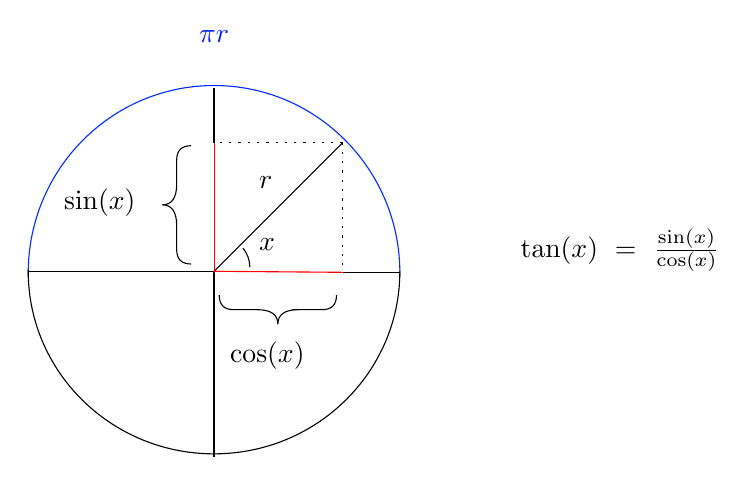
\begin{tikzpicture}[x=0.75pt,y=0.75pt,yscale=-1,xscale=1]
%uncomment if require: \path (0,300); %set diagram left start at 0, and has height of 300

%Straight Lines [id:da7835883213561495] 
\draw    (87,172.89) -- (176.5,172.89) ;
%Straight Lines [id:da2069592864789831] 
\draw    (176.5,262.39) -- (176.5,172.89) ;
%Shape: Arc [id:dp7505851293217748] 
\draw  [draw opacity=0] (87,175.59) .. controls (86.99,174.96) and (86.98,174.33) .. (86.98,173.69) .. controls (86.98,123.82) and (127.06,83.39) .. (176.51,83.39) .. controls (225.95,83.39) and (266.03,123.82) .. (266.03,173.69) .. controls (266.03,174.26) and (266.02,174.82) .. (266.01,175.38) -- (176.51,173.69) -- cycle ; \draw  [color={rgb, 255:red, 0; green, 42; blue, 255 }  ,draw opacity=1 ] (87,175.59) .. controls (86.99,174.96) and (86.98,174.33) .. (86.98,173.69) .. controls (86.98,123.82) and (127.06,83.39) .. (176.51,83.39) .. controls (225.95,83.39) and (266.03,123.82) .. (266.03,173.69) .. controls (266.03,174.26) and (266.02,174.82) .. (266.01,175.38) ;
%Straight Lines [id:da2175596906060845] 
\draw [color={rgb, 255:red, 255; green, 0; blue, 0 }  ,draw opacity=1 ]   (176.5,172.89) -- (238.5,173.39) ;
%Shape: Arc [id:dp9218401449375668] 
\draw  [draw opacity=0] (266.01,172.59) .. controls (266.01,172.69) and (266.02,172.79) .. (266.02,172.89) .. controls (266.02,221.47) and (225.94,260.85) .. (176.5,260.85) .. controls (127.06,260.85) and (86.98,221.47) .. (86.98,172.89) .. controls (86.98,172.68) and (86.99,172.47) .. (86.99,172.26) -- (176.5,172.89) -- cycle ; \draw   (266.01,172.59) .. controls (266.01,172.69) and (266.02,172.79) .. (266.02,172.89) .. controls (266.02,221.47) and (225.94,260.85) .. (176.5,260.85) .. controls (127.06,260.85) and (86.98,221.47) .. (86.98,172.89) .. controls (86.98,172.68) and (86.99,172.47) .. (86.99,172.26) ;
%Straight Lines [id:da791320368124574] 
\draw    (238.5,110.89) -- (176.5,172.89) ;
%Shape: Arc [id:dp7432023456736092] 
\draw  [draw opacity=0] (190.45,161.76) .. controls (192.51,164.24) and (193.75,167.42) .. (193.75,170.89) -- (179.5,170.89) -- cycle ; \draw   (190.45,161.76) .. controls (192.51,164.24) and (193.75,167.42) .. (193.75,170.89) ;
%Straight Lines [id:da5824483322026068] 
\draw [color={rgb, 255:red, 0; green, 0; blue, 0 }  ,draw opacity=1 ] [dash pattern={on 0.84pt off 2.51pt}]  (238.5,110.89) -- (238.5,173.39) ;
%Straight Lines [id:da47524866156438517] 
\draw    (238.5,173.39) -- (266.01,173.39) ;
%Straight Lines [id:da09780504576387938] 
\draw  [dash pattern={on 0.84pt off 2.51pt}]  (238.5,110.89) -- (176.5,110.89) ;
%Straight Lines [id:da3548368319368671] 
\draw [color={rgb, 255:red, 255; green, 0; blue, 0 }  ,draw opacity=1 ]   (176.51,110.89) -- (176.51,132.39) -- (176.51,173.69) ;
%Straight Lines [id:da8124693094798018] 
\draw    (176.5,110.89) -- (176.5,84.39) ;
%Shape: Brace [id:dp5137034581949013] 
\draw   (165.5,112.39) .. controls (160.83,112.39) and (158.5,114.72) .. (158.5,119.39) -- (158.5,130.89) .. controls (158.5,137.56) and (156.17,140.89) .. (151.5,140.89) .. controls (156.17,140.89) and (158.5,144.22) .. (158.5,150.89)(158.5,147.89) -- (158.5,162.39) .. controls (158.5,167.06) and (160.83,169.39) .. (165.5,169.39) ;
%Shape: Brace [id:dp12726316775693558] 
\draw   (179,184.39) .. controls (179,189.06) and (181.33,191.39) .. (186,191.39) -- (197.25,191.39) .. controls (203.92,191.39) and (207.25,193.72) .. (207.25,198.39) .. controls (207.25,193.72) and (210.58,191.39) .. (217.25,191.39)(214.25,191.39) -- (228.5,191.39) .. controls (233.17,191.39) and (235.5,189.06) .. (235.5,184.39) ;

% Text Node
\draw (197,155.79) node [anchor=north west][inner sep=0.75pt]    {$x$};
% Text Node
\draw (103,131.79) node [anchor=north west][inner sep=0.75pt]    {$\sin( x)$};
% Text Node
\draw (197,125.79) node [anchor=north west][inner sep=0.75pt]    {$r$};
% Text Node
\draw (183,205.79) node [anchor=north west][inner sep=0.75pt]    {$\cos( x)$};
% Text Node
\draw (168,55.79) node [anchor=north west][inner sep=0.75pt]  [color={rgb, 255:red, 0; green, 24; blue, 255 }  ,opacity=1 ]  {$\pi r$};
% Text Node
\draw (323,151.4) node [anchor=north west][inner sep=0.75pt]    {$\tan( x) \ =\ \frac{\sin( x)}{\cos( x)}$};


\end{tikzpicture}